\documentclass{article}
\usepackage[utf8]{inputenc}
\usepackage{url}
\usepackage[margin=0.75in]{geometry}
\usepackage{float}
\usepackage{graphicx}
\usepackage{longtable}

\setlength{\parskip}{0.7em}
\setlength{\parindent}{0em}

\begin{document}
	\begin{center}
    
    	% MAKE SURE YOU TAKE OUT THE SQUARE BRACKETS
		\LARGE{\textbf{CSE 6730, Group 37 Final Report}} \\
        \vspace{1em}
        \Large{Discrete Event Simulation} \\
     
	\end{center}
    \begin{normalsize}
    
    	\section{Project Title}
        
Simulation of the Spread of Syphilis within Group Housing for the Elderly
      
		\section{Team Members}
        
      \begin{enumerate}
      	\item Aiswarya Bhagavatula (GTID 903540374)
      	\item D. Aaron Hillegass (GTID 901988533)
      	\item Siawpeng Er (GTID 903413430)
      	\item Xiaotong Mu (GTID 903529807)
      \end{enumerate}
        
	   	\section{Problem Description and Purpose}
        
    More and more communities of the elderly are suffering from outbreaks of sexually transmitted infections \cite{mcdaniel_2017}. According to Athena Health, patients over 60 account for the biggest increase of in-office treatments for sexually transmitted infections.
    
    For this study, we are going to focus on syphilis, but the methodology and resulting simulation could easily be applied to other treatable, non-deadly STIs like chlamydia and gonorrhea.
    
    There are several factors that have led to the spread of STIs among older people (especially in group housing):
    \begin{itemize}
	\item Lack of safer sex practices (such as condom use) in older individuals. People who became sexually active before AIDS are less likely to follow safe sex practices.
    \item Imbalances between the number of men and women. In retirement homes, there are typically significantly more women than men. It would not be surprising to find that the few healthy men would act as a nexus for sexually transmitted infections.
    \item Shame around testing and treatment. Older people (especially married older people) might be reluctant to tell their doctor about symptoms, get tested, and pursue treatment.
    \item Number of opportunities for transmission. In earlier times, we could expect sexual activity to diminish in the aging population.  However, with people living longer, healthier lives and the proliferation of safe erectile dysfunction drugs, people in retirement communities are more sexually active than their parents were at the same age -- especially if they live in close community with a large number of potential partners.
    \item Antibiotic resistance. Old people living in community are likely to get other kinds of bacterial infections, like strep, and take antibiotics. In the past, this was likely to wipe out undiagnosed syphilis (or chlamydia or gonorrhea) as a side-effect. As these STIs have evolved to become more antibiotic resistant, a strep-sized dose of amoxicillin is less likely to do the job.
    \end{itemize}
    
    Discrete Event Simulation (DES) was been used for long time in many healthcare simulation, ranging from health care system operation, disease progression modeling, screening modeling and health behavior modeling \cite{lebcir2017, Zhang2018}. 
    
    
     A realistic simulation of the transmission of STIs in retirement homes could be useful in deciding between different interventions.  For example, would increasing condom use by 20\% be more effective than annual STI tests?
       
     \section{Literature review}
     Propagation of Sexually transmitted diseases (STD) is modelled mainly based on the option of the social network that describes the contact between individuals. Perhaps the initial form of these models was STDSIM, created in the late 1990s and utilised in numerous HIV modelling studies \cite{10.2307/25062378}.
     
     The network models have become increasingly difficult with the use of information from the populaces under examination. One such model depicts a collection of work around demonstrating the HIV pandemic in Vancouver, which incorporates a system model of infusing drug clients and female sex laborers, with the point of evaluating the viability of various control methodologies. 
     
     To model STDs, a network model is generated with an analogy of vertices representing persons and edges representing contacts.A transmission event can happen in cases of connected edges, thus making the probability distribution of the number of edges of each node a very salient feature. Each of the edges can have various weights which directly relate to the type of interactions between the individuals. For instance, the netwrok can be modeled in three levels of interactions that determine heterosexual contact:0, no contact; 1, spousal partnership; 2, non-spousal partnership \cite{c030e9dad6134c6e9a9d18e61b852e99}.


	Although, this can be very difficult in cases with large datasets as developing models with social networks would need a large number of people to have expertise on the different fields involved like statistics, computer science, ethnography, medicine among others. 
	
	An alternative model can be built by considering mainly a few concise statistics regarding the extensive data \cite{dataset}. These contact networks make way for analysing the break of disease transmissions between persons by the use of condoms and other precautionary measures. This helps understand the impact of superspreaders as well. There are other models of STDs that are based on System Dynamics and other concepts. These are mainly aimed for making decisions on how to allocate resources to reduce STDs in a targeted testing program \cite{Kok2015}.

     \section{Data source}
    We get the data from the Centers for Disease Control and Prevention (CDC) website for parameters on syphilis. This includes:
    \begin{itemize}
    \item Rates in the general population at the ages at which people would enter retirement homes
   	\item Likelihood of transmission for different types of sexual activity (intercourse, oral, anal).
   	\item Time after infection before symptoms appear.
   	\end{itemize}
   	
   	We will also use a local retirement community to be modeled. From that administration we will find out:
   	\begin{itemize}
    \item Number of men and women 
    \item Ages at which people enter the community
    \item Duration that people stay in the community
    \item What, if any, STI testing and treatment are provided to the residents
   	\end{itemize}     
   	
   	Finally, we will do some interviews with residents to create a model of the individual:
   	\begin{itemize}
    \item Number of sexual partners per year
    \item History of STI testing and treatment 
    \item Marital status
    \item Gender
    \item Age
    \item Types of sexual activity that they engage in (if possible)
   	\end{itemize}     
   	
 We successfully obtained the real data about syphilis directly from the CDC through some connections.
 
 From the data obtained, we cross checked with some literature review and come out with the distribution as Table \ref{tab:parameter}. Furthermore, from the population, we obtain the mean and the standard deviation on the age and the gender. By doing this, when we randomly generate the residents for our simulation, it will be closer to the data obtained. Since this is relatively easy probability (ratio of the gender, age), we do not found any abnormalities in the generated data.
   	
   	\section{Methodology}
   	Our simulation will first simulate a population of people entering and exiting a single retirement community. It will use stochastic methods to give them an initial age, gender, and infection status.  It will also remove these people as move somewhere else or die. When someone dies or moves away, this creates room for a new resident.
   	
   	Within that population, we will update each individual's infection status as they become infected and get treated. We will also track if they have become symptomatic. Thus, each time an uninfected person engages in sexual activity with an infected person, we will roll the dice to decide if the uninfected person becomes infected. Each person will be symptomatic for some amount of time before seeking testing and treatment.
   	
   	We will test different interventions:
   	\begin{itemize}
    \item Increasing condom usage
    \item Periodic testing and treatment of the whole community 
    \item Promoting monogamous fluid bonding
	\item Working toward equal numbers of men and women in the community
   	\end{itemize}     
    
    \section{Modelling using Discrete Event Simulation}
	Discrete event simulation is a form of computer based modelling that provides an intuitive and flexible approach to representing complex systems. Our model simulates the dynamics of main, and casual sexual partnerships, with behavioural model parameters estimated form sexual network data.
	
	\subsection{Structural development}
	The core concepts of DES are entities, attributes, events, resources, queues, and time. In disease modeling studies, the network model will generally consist of a set of individuals connected by contacts, where it is assumed that the contacts are such that if a transmission event could take place. The use of the most important feature is how well individuals are connected. In pair-formation models developed by Dietz and Hadeler, Waldstätter, and Kretzschmar and Dietz \cite{dietz_hadeler_1988} ,the pair-formation framework allow modeling of differential infection risk among persons who are single or paired, and it has been widely used in a number of other mathematical models of sexually transmitted infections \cite{heijne_althaus_herzog_kretzschmar_low_2011, powers_ghani_miller_hoffman_pettifor_kamanga_martinson_cohen_2011,xiridou_geskus_wit_coutinho_kretzschmar_2003, ferguson_garnett_2000}.
	
	Our model include compartments that stratify the population by age, sex, partnership status, sexual risk behavior, and infection status. Transmission of sexual disease in the model occurs via unprotected sex in heterosexual partnerships (refer to Fig. \ref{fig:blockDiagram})
	
	Predictors of partnership formation varies by partnership type,risk level,, age mixing, and status-unknown partnership. In our model, there are 2 partnership statuses that are mutually exclusive. Entity can be part of the unpaired(“single”)population or paired(“married”), unpaired population can have casual partners at age-specific rates. Casual partners represent short term relationships, and they are modeled as instantaneous partnerships. Behavioral parameters were informed by the National Survey of Family Growth. Parameters and their prior distributions \cite{galer_et2019} are shown in Table \ref{tab:parameter}. 
	
	
	\begin{table}[H]
	\centering
    	\begin{tabular}{ |p{5cm}|p{7cm}|p{5cm}| } 
    		\hline
    		Parameter/Variable & Description & Distribution  \\ 
    		\hline
    		Population size & Population size for each age group & Uniformly distributed\\
    		Time step &	Time step implemented in the model & 	A day \\
			High risk & Fraction of the population defined as high risk	& 10\% (Assumption) \\
			Low risk & Fraction of the population defined as low risk & 90\% (Assumption)\\
			\hline
			\multicolumn{3}{|c|}{Testing symptomatic individuals} \\
			\hline
			Women &	Testing of symptomatic  women	& 1/(52*(0.079+0.072*Beta(4,4)))\\
			Men	& Testing of symptomatic men	& 1/(52*(0.079+0.072*Beta(4,4)))\\
			\hline
			\multicolumn{3}{|c|}{Casual partners} \\
			\hline
			High risk(HR)& Single, 65-79 HR	& Beta(3,60)\\
 						 & Single, 80-95 HR	& Beta(3,400)\\
			Low risk(LR)	 & Single, 65-79 LR	& Beta(1,160) \\
 						 & Single, 80-95 LR	&Beta(1,160)\\
 			\hline
 			\multicolumn{3}{|c|}{Among paired} \\
 			\hline
			High risk(HR)& Single, 65-79 HR	& Beta(10,70)\\
			Low risk(LR) & Single, 80-95 LR	& Beta(10,100)\\
			Treatment success(efficiency of antibiotics)	 & & Beta(190,8)\\
			\hline
			\multicolumn{3}{|c|}{Natural recovery} \\
			\hline
			Women & & 1/(52*(1.13+0.5*Beta(4,4.969)))\\
			Men & & 1/(52*(1.13+0.5*Beta(4,4.969)))\\
			Transmission probability	 & Per act probability	& Beta(5.5, 50)\\
    		\hline
    	\end{tabular}
    	
    	\caption{Description of parameters governing testing, natural recovery and transmission probability}
    	\label{tab:parameter}
   \end{table}
   
   	we chose to fix the fraction of the population defined as high risk at constant 10\%, but accommodate uncertainty in levels of risk behavior by varying the partner change rates by relationship states and age, in each of the risk groups. Defining a set proportion of the population to belong to a risk group and varying partner change rates is a modeling convention

\begin{figure}[H]
\caption{Block Diagram of  the Simulation}
\centering
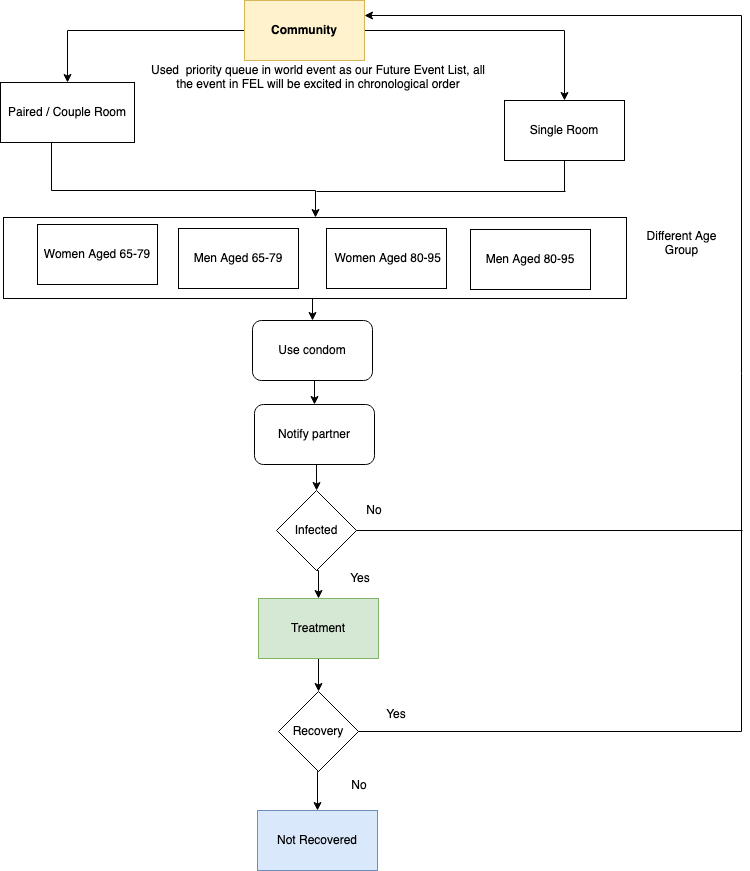
\includegraphics[width=1\textwidth]{BlockDiagram.png}
\label{fig:blockDiagram}
\end{figure}


    \section{Development Platform}
    The programming language is Python $3$. Depends on the suitability of the project, we plan to provide a Jupyter notebook for user interaction, or just a command line execution.
    
    We will use heapq as our priority queue. This priority queue is also our future event list (FEL) in our simulation event. All the events will be sent to here and execute according to chronological order.
     
	\subsection{Development}
	In our final software, we successfully create a one priority queue future event list (FEL) based discrete event simulation (DES).  
	We have successfully model the World as our simulation environment. We have a set of parameters as per Table \ref{tab:parameter2} with their corresponding description.
	
	As a brief description of our system, we simulated a elderly house based on the data we obtained to get the population distribution of the residents involved. Room will be allocated to the residents, according to couple or just some single room, we simulate sometime some single room will be occupied with more than $1$ person of different gender to simulate a possible sexual activity event.
	
	Upon sexual activity event, there are different probability for each group of residents to get affected in sexually transmitted infection (STI), and in our case, Syphillis. The probability distributions are according to the literature review. $2$ interventions could be done during this phase, namely whether the parties involved use condom, or they notify their partner if have STI. Such intervention may decrease the chance of affection.
	
	Each sexual activity may result in sexually transmitted disease (STD) with our focus on Syphilis. We have two treatment option, whether to do antibiotics treatment, or just allow the patients to recover naturally. These two treatment options may affected the chance of recovery.
	     
    \begin{table}[H]
	\centering
    	\begin{tabular}{ |p{5cm}|p{7cm}| } 
    		\hline
    		Parameters & Description\\
    		\hline
    		\multicolumn{2}{|c|}{General} \\
    		\hline
    		logfile & logfile name\\
    		room\_cluster\_count & number of cluster\\
    		room\_per\_cluster\_count & number of room per cluster\\
    		prob\_new\_room\_for\_married & probability of the room as couple room\\
    		prob\_new\_single\_male & probability of a new single male\\
    		max\_age\_male\_resident & maximum age of male resident\\
    		max\_age\_female\_resident & maximum age of female resident\\
    		mean\_age\_new\_resident & the mean age of the new resident\\ 
    		sd\_age\_new\_resident & standard deviation of the age of new resident\\
    		max\_day\_room\_empty & maximum number the room is not occupied\\
   			\hline
   			\multicolumn{2}{|c|}{Infection risk} \\
   			\hline
   			HR & high risk probability\\
   			LR & low risk probability\\
   			std\_probability & all other group member not covered belong to here\\
   			std\_with\_condom & probability with infection using condom\\
   			std\_without\_condom & probability with infection without using condom\\
   			\hline
   			\multicolumn{2}{|c|}{Infection risk with casual partner} \\
   			\hline
   			casual\_std\_65\_79\_HR & probability of infection for high risk group with age 65 to 79\\
   			casual\_std\_80\_95\_HR & probability of infection for high risk group with age 80 to 95\\
   			casual\_std\_65\_79\_LR & probability of infection for low risk group with age 65 to 79\\
   			casua\_std\_80\_95\_LR & probability of infection for low risk group with age 80 to 95\\
    		\hline
    		\multicolumn{2}{|c|}{Infection risk among couple} \\
    		\hline
    		casual\_std\_65\_79\_HR & probability of infection for high risk group with age 65 to 79\\
    		casual\_std\_80\_95\_LR & probability of infection for low risk group with age 80 to 95\\
    		\hline
    		\multicolumn{2}{|c|}{Intervention method} \\
    		\hline
    		use\_condom & whether to promote using condom\\
    		notify\_partner & whether to promote notify partner if get affected\\
    		notification & change of notification\\
    		condom\_casual\_partner & how likely to use condom among casual partners\\
    		condom\_paired\_partner & how likely to use condom among couple\\
    		\hline
    		\multicolumn{2}{|c|}{Treatment method} \\
    		\hline
    		choice\_of\_treatment & choose between "antibiotics" or "natural recovery"\\
    		woman\_nr & female probability of recovery when just using natural recovery\\
    		man\_nr & male probability of recovery when just using natural recovery\\
    		antibiotics & probability of recovery when using antibiotics\\
    		\hline
    	\end{tabular}
  
    	\caption{Description of parameters in the simulation}
    	\label{tab:parameter2}
   \end{table}

\section{Simulation result}
While our model is flexible and could include more variable under testing, we wish to focus on our investigation on $2$ intervention and $2$ treatment condition. Our intervention include: $1.$ Using condom, $2.$ Notify partner whenever you might have STI. For our treatment, it is either $1.$ antibiotics or $2.$ natural recovery, equivalent to no treatment.

Different scenarios of simulation was run as per below:

	\begin{enumerate}
		\item Natural recovery, not using condom, not notify partner
		\item Natural recovery, using condom, not notify partner
		\item Natural recovery, not using condom, notify partner
		\item  Natural recovery, using condom, notify partner
		\item Antibiotics, not using condom, not notify partner
		\item  Antibiotics, using condom, notify partner
	\end{enumerate}


We run the simulation each for $30$ times and summarized as in Table \ref{tab:result} below. The reason for using $30$ time simulation is to ensure the result is statistically significant, according to the Law of Large Number. We further summarize mean, standard error, standard deviation, and 95\% CI for each of the  simulation data and show in Table \ref{tab:result2}.

\begin{longtable}{|p{7cm}|p{7cm}|}
		\hline
		Parameters  & Number of residents\\ 
		\hline
		\multicolumn{2}{|c|}{Simulation Type $1$} \\
		\multicolumn{2}{|c|}{Treatment involved : natural recovery} \\
		\multicolumn{2}{|c|}{Intervention involved : use condom: no} \\
		\multicolumn{2}{|c|}{Intervention involved : notification of partner: no} \\
		\hline
		Total male & 58.33\\
		Total female & 77.47\\
		Total couple & 46.30\\
		Healthy male & 25.87\\
		Healthy female & 44.53\\
		Infected male: & 33.63\\
		Infected female: & 33.67\\
		Total male recovered & 0.67\\
		Total female recovered & 0.73\\
		\hline
		\multicolumn{2}{|c|}{Simulation Type $2$} \\
		\multicolumn{2}{|c|}{Treatment involved : natural recovery} \\
		\multicolumn{2}{|c|}{Intervention involved : use condom: yes} \\
		\multicolumn{2}{|c|}{Intervention involved : notification of partner: no} \\
		\hline
		Total male & 59.77\\
		Total female & 76.67\\
		Total couple & 46.43\\
		Healthy male & 51.90\\
		Healthy female & 66.86\\
		Infected male: & 8.16\\
		Infected female: & 10.13\\
		Total male recovered & 0.30\\
		Total female recovered & 0.33\\	
		\hline
		\multicolumn{2}{|c|}{Simulation Type $3$} \\
		\multicolumn{2}{|c|}{Treatment involved : natural recovery} \\
		\multicolumn{2}{|c|}{Intervention involved : use condom: no} \\
		\multicolumn{2}{|c|}{Intervention involved : notification of partner: yes} \\
		\hline
		Total male & 58.63\\
		Total female & 76.70\\
		Total couple & 45.33\\
		Healthy male & 44.13\\
		Healthy female & 63.03\\
		Infected male: & 14.70\\
		Infected female: & 13.93\\
		Total male recovered & 0.20\\
		Total female recovered & 0.37\\		
		\hline
		\multicolumn{2}{|c|}{Simulation Type $4$} \\
		\multicolumn{2}{|c|}{Treatment involved : natural recovery} \\
		\multicolumn{2}{|c|}{Intervention involved : use condom: yes} \\
		\multicolumn{2}{|c|}{Intervention involved : notification of partner: yes} \\
		\hline
		Total male & 60.50\\
		Total female & 75.40\\
		Total couple & 45.90\\
		Healthy male & 57.50\\
		Healthy female & 71.76\\
		Infected male: & 3.17\\
		Infected female: & 3.67\\
		Total male recovered & 0.17\\
		Total female recovered & 0.03\\		
		\hline
		\multicolumn{2}{|c|}{Simulation Type $5$} \\
		\multicolumn{2}{|c|}{Treatment involved : antibiotics} \\
		\multicolumn{2}{|c|}{Intervention involved : use condom: no} \\
		\multicolumn{2}{|c|}{Intervention involved : notification of partner: no} \\
		\hline
		Total male & 59.23\\
		Total female & 77.07\\
		Total couple & 46.30\\
		Healthy male & 58.90\\
		Healthy female & 76.73\\
		Infected  male: & 34.00\\
		Infected female: & 33.67\\
		Total male recovered & 33.67\\
		Total female recovered & 33.33\\		
		\hline
		\multicolumn{2}{|c|}{Simulation Type $6$} \\
		\multicolumn{2}{|c|}{Treatment involved :antibiotics} \\
		\multicolumn{2}{|c|}{Intervention involved : use condom: yes} \\
		\multicolumn{2}{|c|}{Intervention involved : notification of partner: yes} \\
		\hline
		Total male & 60.63\\
		Total female & 76.03\\
		Total couple & 46.67\\
		Healthy male & 60.53\\
		Healthy female & 75.83\\
		Infected male: & 3.20\\
		Infected female: & 4.13\\
		Total male recovered & 3.10\\
		Total female recovered & 3.93\\
		\hline
	\caption{Result of simulation}
	\label{tab:result}
\end{longtable}

\begin{longtable}{|p{5cm}|p{3cm}|p{3cm}|p{3cm}|p{3cm}|}
	\hline
	Parameters  & Mean & Standard Error & Standard Deviation & Confidence Level (95\%)\\ 
	\hline
	\multicolumn{5}{|c|}{Simulation Type $1$} \\
	\multicolumn{5}{|c|}{Treatment involved : natural recovery} \\
	\multicolumn{5}{|c|}{Intervention involved : use condom: no} \\
	\multicolumn{5}{|c|}{Intervention involved : notification of partner: no} \\
	\hline
	Total male & 58.33 &  0.77 & 4.21 & 1.57\\
	Total female & 77.47 & 0.73 & 4.02 & 1.50\\
	Total couple & 46.30 & 0.92 & 5.07 & 1.89 \\
	Healthy male & 25.87 & 0.92 & 5.02 & 1.88 \\
	Healthy female & 44.53 & 0.82 & 4.52 & 1.69 \\
	Infected male: & 33.63 & 1.01 & 5.55 & 2.07 \\
	Infected female: & 33.67 & 0.83 & 4.56 & 1.70\\
	Total male recovered & 0.67 & 0.12 & 0.66 & 0.25\\
	Total female recovered & 0.73 & 0.14 & 0.74 & 0.28\\
	\hline
	\multicolumn{5}{|c|}{Simulation Type $2$} \\
	\multicolumn{5}{|c|}{Treatment involved : natural recovery} \\
	\multicolumn{5}{|c|}{Intervention involved : use condom: yes} \\
	\multicolumn{5}{|c|}{Intervention involved : notification of partner: no} \\
	\hline
	Total male & 59.77 & 0.87 & 4.79 & 1.79 \\
	Total female & 76.67 & 0.61 & 3.35 & 1.25 \\
	Total couple & 46.43 & 0.83 & 4.53 & 1.69\\
	Healthy male & 51.90 & 1.03 & 5.65 & 2.11\\
	Healthy female & 66.86 & 0.72 & 3.93 & 1.47 \\
	Infected male: & 8.16 & 0.64 & 3.50 & 1.31\\
	Infected female: & 10.13 & 0.49 & 2.67 & 1.00\\
	Total male recovered & 0.30 & 0.09 & 0.47 & 0.17\\
	Total female recovered & 0.33 & 0.11 & 0.61 & 0.23\\	
	\hline
	\multicolumn{5}{|c|}{Simulation Type $3$} \\
	\multicolumn{5}{|c|}{Treatment involved : natural recovery} \\
	\multicolumn{5}{|c|}{Intervention involved : use condom: no} \\
	\multicolumn{5}{|c|}{Intervention involved : notification of partner: yes} \\
	\hline
	Total male & 58.63  & 0.59 & 3.23 & 1.20\\
	Total female & 76.70 & 0.55 & 3.02 & 1.13\\
	Total couple & 45.33 & 0.76 & 4.19 & 1.56\\
	Healthy male & 44.13 & 0.64 & 3.51 & 1.31\\
	Healthy female & 63.03 & 0.69 & 3.76 & 1.41\\
	Infected male: & 14.70 & 0.47 & 2.55 & 0.95\\
	Infected female: & 13.93 & 0.59 & 3.23 & 1.20\\
	Total male recovered & 0.20 & 0.07 & 0.41 & 0.15\\
	Total female recovered & 0.37 & 0.10 & 0.52 & 0.19\\		
	\hline
	\multicolumn{5}{|c|}{Simulation Type $4$} \\
	\multicolumn{5}{|c|}{Treatment involved : natural recovery} \\
	\multicolumn{5}{|c|}{Intervention involved : use condom: yes} \\
	\multicolumn{5}{|c|}{Intervention involved : notification of partner: yes} \\
	\hline
	Total male & 60.50 & 0.91 & 4.97 & 1.85\\
	Total female & 75.40 & 0.58 & 3.16 & 1.18\\
	Total couple & 45.90 & 0.83 & 4.57 & 1.71\\
	Healthy male & 57.50 & 1.04 & 5.68 & 2.12\\
	Healthy female & 71.76 & 0.59 &  3.22 & 1.20\\
	Infected male: & 3.17 & 0.36 & 1.95 & 0.73\\
	Infected female: & 3.67 & 0.41 & 2.23 & 0.83\\
	Total male recovered & 0.17 & 0.07 & 0.38 & 0.14 \\
	Total female recovered & 0.03 & 0.03 & 0.18 & 0.07\\		
	\hline
	\multicolumn{5}{|c|}{Simulation Type $5$} \\
	\multicolumn{5}{|c|}{Treatment involved : antibiotics} \\
	\multicolumn{5}{|c|}{Intervention involved : use condom: no} \\
	\multicolumn{5}{|c|}{Intervention involved : notification of partner: no} \\
	\hline
	Total male & 59.23 & 0.95 & 5.21 & 1.95\\
	Total female & 77.07 & 0.68 & 3.72 & 1.39\\
	Total couple & 46.30 & 0.89 & 4.85 & 1.81\\
	Healthy male & 58.90 & 0.94 & 5.16 & 1.92\\
	Healthy female & 76.73 & 0.71 & 3.91 & 1.46\\
	Infected  male: & 34.00 & 0.90 & 4.93 & 1.84\\
	Infected female: & 33.67 & 0.90 & 4.95 & 1.84\\
	Total male recovered & 33.67 & 0.92 & 5.04 & 1.88\\
	Total female recovered & 33.33 & 0.90 & 4.94 & 1.85\\		
	\hline
	\multicolumn{5}{|c|}{Simulation Type $6$} \\
	\multicolumn{5}{|c|}{Treatment involved :antibiotics} \\
	\multicolumn{5}{|c|}{Intervention involved : use condom: yes} \\
	\multicolumn{5}{|c|}{Intervention involved : notification of partner: yes} \\
	\hline
	Total male & 60.63 & 0.73 & 4.00 & 1.50\\
	Total female & 76.03 & 0.63 & 2.47 & 1.30\\
	Total couple & 46.67 & 0.91 & 4.96 & 1.85\\
	Healthy male & 60.53 & 0.75 & 4.11 & 1.53\\
	Healthy female & 75.83 & 0.63 & 3.48 & 1.30\\
	Infected male: & 3.20 & 0.31 &1.71 & 0.64\\
	Infected female: & 4.13 & 0.46 & 2.53 & 0.94\\
	Total male recovered & 3.10 & 0.32 & 1.73 & 0.65\\
	Total female recovered & 3.93 & 0.48 & 2.49 & 0.91\\
	\hline
	\caption{Result of simulation - Mean, Standard Error, Standard Deviation and 95\% Confidence Interval for each simulation}
	\label{tab:result2}
\end{longtable}

From the result above, we could see without intervention and treatment, it is high vulnerable for the residents on the STI. Moreover, their recovery is really bad. This is shown in Simulation type $1$. 

When we investigate different effect from the using condom and notification of partner, and their combine effect. We could see any of the intervention is effective, as shown in Simulation type $2$, $3$, and $4$. In effect, notification of partner highly prevent any sexual activity, so only a few residents get infected. For the effective usage of condom, the effect is the same, and preventing residents from infected by STI.

When antibiotics was introduced, the recovery rate is very promising, as shown in Simulation type $5$. However, the antibiotics treatment may be expensive and most elderly housing has no financial capability to do so. In Simulation type $6$, we see both the recovery rate and the infection rate drop when both the intervention methods and antibiotics treatment are implemented. From the financial point of view, using intervention could help to release some of the financial burden from the administrative party for the elderly house. On the other hand, by always resorting to antibiotics treatment for the infected residents could help them to recover from the STI.

\section{Verification and Validation}
\subsection{Assumptions}
\begin{itemize}
	\item No age mixing input preference
	\item Partner notification is stratified by sex and age, however in the absence of data on changes in this prevention strategy, the parameters are kept time invariant
	\item Only heterosexual partnerships.
	\item Treatment ensued immediately following identification of infection, although this may not always happen in practice.
\end{itemize}
Furthermore, probability distribution of the parameters used in our model is shown in Table \ref{tab:parameter3}\\
	\begin{table}[H]
	\centering
	\begin{tabular}{ |p{5cm}|p{7cm}|p{5cm}| } 
		\hline
		Parameter/Variable & Description & Distribution  \\ 
		\hline
		Population size & Population size for each age group & Uniformly distributed\\
		Time step &	Time step implemented in the model & 	A day \\
		High risk & Fraction of the population defined as high risk	& 10\% (Assumption) \\
		Low risk & Fraction of the population defined as low risk & 90\% (Assumption)\\
		\hline
		\multicolumn{3}{|c|}{Testing symptomatic individuals} \\
		\hline
		Women &	Testing of symptomatic  women	& 1/(52*(0.079+0.072*Beta(4,4)))\\
		Men	& Testing of symptomatic men	& 1/(52*(0.079+0.072*Beta(4,4)))\\
		\hline
		
		\multicolumn{3}{|c|}{Casual partners} \\
		\hline
		High risk(HR)& Single, 65-79 HR	& Beta(3,60)\\
		& Single, 80-95 HR	& Beta(3,400)\\
		Low risk(LR)	 & Single, 65-79 LR	& Beta(1,160) \\
		& Single, 80-95 LR	&Beta(1,160)\\
		\hline
		\multicolumn{3}{|c|}{Among paired} \\
		\hline
		High risk(HR)& Single, 65-79 HR	& Beta(10,70)\\
		Low risk(LR) & Single, 80-95 LR	& Beta(10,100)\\
		\hline
		
		\multicolumn{3}{|c|}{Transmission: This value will multiply with the original risk} \\
		\hline
		Transmission probability & Per act probability & 1\\
		With condom protection & condom effect parameter estimate is reducing 50\% of transmission& 0.5\\
		\hline
		
		\multicolumn{3}{|c|}{Natural recovery} \\
		\hline
		Women & & 1/(52*(1.13+0.5*Beta(4,4.969)))\\
		Men & & 1/(52*(1.13+0.5*Beta(4,4.969)))\\
		
		\hline
		
		\multicolumn{3}{|c|}{Treatment Success} \\
		\hline
		Efficiency of antibiotics & & Beta(190,8)))\\
		\hline
		
		\multicolumn{3}{|c|}{Partner Notification} \\
		\hline
		Women&Age65-79&Beta(4,3)\\
		&Age80-95&Beta(4,3)
		\\
		Men&Age65-79&Beta(4,3)\\
		&Age80-95&Beta(4,3)\\
		\hline
		\multicolumn{3}{|c|}{Condom Use} \\
		\hline
		Casual partners&Weighted prevalence & 0.131\\
		Paired & Weighted prevalence & 0.368
		\\
		\hline
			
		% https://www.ncbi.nlm.nih.gov/pmc/articles/PMC5477642/
		
	\end{tabular}

	\caption{Description of parameters governing testing, natural recovery and transmission probability}
	\label{tab:parameter3}
\end{table}

\subsection{Verification}
Our conceptual model is based on the workflow in Figure \ref{fig:blockDiagram}. At the beginning, we initiate the Simulation World and allow the residents to be occupied in the room. Typically, room could be divided into two types: paired/couple room, or single room. For single room, sometime it could resides more people of different gender. This is our simplified model of interaction between affected couple.

Subsequently, sexual event may occurs betwee resident of different sex. Based on their age and room type, we assigned different risk to them. The risk will be further augmented or decreased by the usage of condom and whether they notify their partners on their possibilities of getting STI.

Once infected with the STI, they may be treated. The treatment may be antibiotics or natural recovery (which is equivalent to no treatment). Upon recovery, they are back to the community, else they will be logged as infected patients.

In our simulation model, the model was done according to the conceptual model according to the flow chart as described above. Moreover, for repeatability, we set our seed according to the number of the simulation we are currently run. The result are recorded in CSV file for checking of our assumptions and our conceptual model. 

\subsection{Validation}
\textbf{Comparison to other model:}\\

To explore the impact of partner notification and condom effectiveness on sexually disease transmission. we calibrated the model under 4 discrete scenarios, For quantification of the overall impact, we ran 30 replications for each scenario, and compute the average for each. the first scenario analysis assumed that there was no condom or partner notification ; the second scenario assumed that there was no partner notification for the time period; the third scenario analysis assumed that there was no condom used; The fourth scenario included both interventions.\\


\begin{figure}[H]
\caption{Estimated Impact of Using condom and partner notification}
\centering
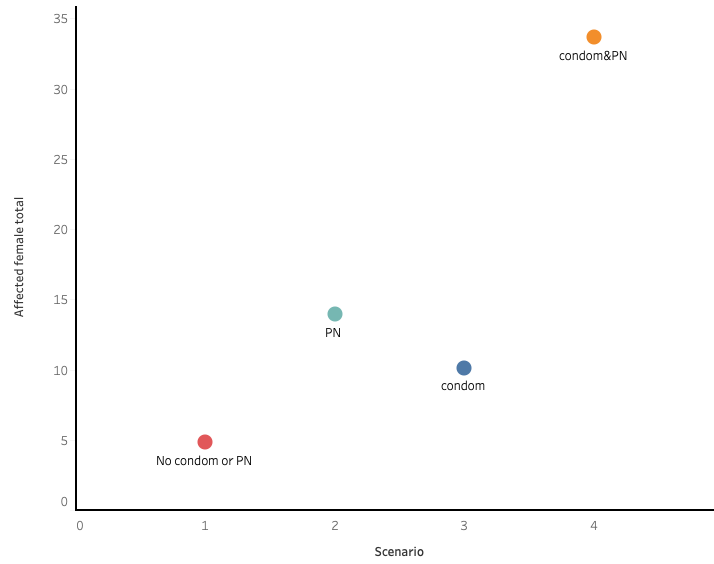
\includegraphics[width=0.6\textwidth]{plt1.png}
\label{fig:plt1}
\end{figure}

\begin{figure}[H]
\caption{Estimated Impact of Using condom and partner notification}
\centering
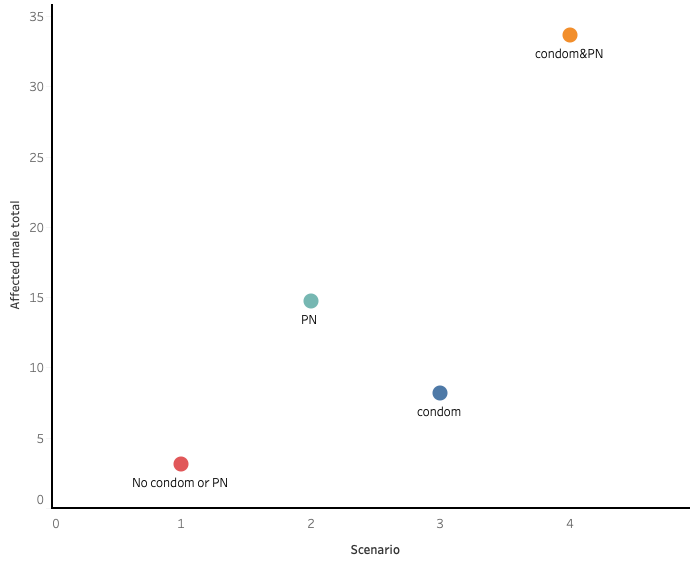
\includegraphics[width=0.58\textwidth]{plt3.png}
\label{fig:plt4}
\end{figure}


\begin{figure}[H]
\caption{Estimated Impact of Using condom and partner notification}
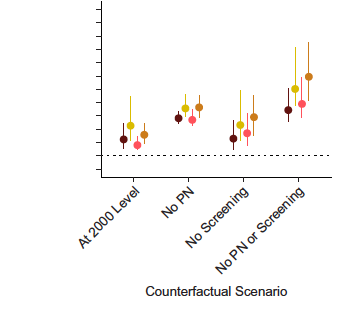
\includegraphics[width=0.83\textwidth]{plt2.png}
\label{fig:plt2}
\end{figure}


 For the same time period, national prevalence estimates from the National Health and Nutrition Examination Survey lacked a clear trend, and the estimates were characterized by wide confidence intervals in Figure 3. The high variability does not effect our simulation model, because all the variables are randomly generated with fix distribution. 
 In our simulation model, instead of exploring the impact of uncertainty regarding trends in screening and reporting, we would like to learn more about the effect of condom use on sexual disease transmission. Because part of the reason these bacterial sexually transmitted infections are so common is that they are really contagious.
 How ever the efficacy of condoms for protection against transmission has not previously measured on a per act basis, because the measured correct use and condom use problems could introduce bias resulting in condom effectiveness similar to that produced by combining consistent and inconsistent users.
 We examined the efficacy of condom use in prevention simplex virus type 2(HSV-2)transmission. By comparing the number of transmissions per 1000 unprotected acts and protected acts, the condom use reduced the per-act probability of transmission by 65\%, to avoid overestimating the effectiveness of condom use, we used 50\% * original transmission prob if condom used. \\
 

 
 As we can see from Figure 2, each of the 4 scenarios produced joint posterior estimates of the model consistent with the observed epidemiologic data[Figure 3]. Absence of both using condom and partner notification had the largest impact on estimated prevalence for both sex. The modeling results suggested that the greatest impact in STD prevention has come from combining condom use with partner notification.\\
 
\textbf{Degenerate Tests and Sensitivity Analysis:}\\

Untreated patients with STD infection can contribute to continued disease transmission in the community. For many types of sexually transmitted infections (STDs) patients should administer appropriate therapy to prevent this transmission. \\

 Treatment is critical, it is a rate-limiting. As shown in Figure 5, with treatment, there is a huge improvement in the number of recovered patients. Furthermore, It has the highest impact on the first scenario which has no condom use and partner notification. In the first scenario, patients have a higher probability of acquiring STD from and infected source, thus the number of people recovered are greater.  Our review leads to the recommendation that if the patient is infected, the partner(s) should be treated as well to prevent reinfection and further spread of the disease.
 
\begin{figure}[H]
\caption{Effect of Treatment in Different Scenario}
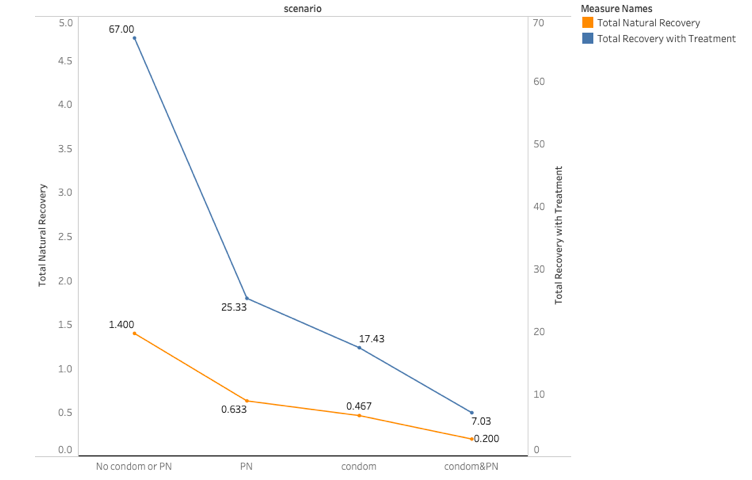
\includegraphics[width=0.8\textwidth]{plt4.png}
\centering
\label{fig:plt4}
\end{figure}


\textbf{Extreme Condition Tests:}\\

To further validate our model, we look at the model structure and outputs for extreme and unlikely combination of levels of factors in the system. Assume no treatment ad partner notification,we ran our simulation model with different probability of getting infected when condoms are used. As we can observe in Figure 6, when condoms have perfect efficacy for protection against STDs, no people get infected. as the efficacy decreases, the number of infected patients increases, and eventually it converges to the number of infected patients in the scenario without condom use.\\ 

Condoms are recommended as an effective preventive method for heterosexual transmission. However, the exact magnitude of risk reduction is difficult to quantify because of limitations and variations in the methods and design of these studies. The 2 largest issues remain how best to measure condom use and how best to identify study populations with documented exposure to infection. 

\begin{figure}[H]
\caption{Effect of Condom Use on Infected Total }
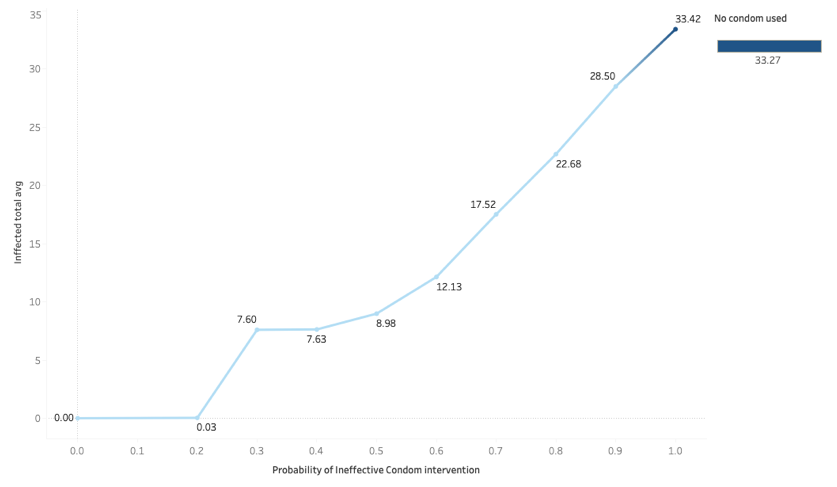
\includegraphics[width=0.8\textwidth]{plt5.png}
\centering
\label{fig:plt4}
\end{figure}

\subsection{Future work}
Our model in this project is relatively simple. While it fit our purpose of simulation, we could further improve it in future work.
Several of the improvement that we think could be further improved:
\begin{itemize}
	\item More type of STI\\
	Currently, only Syphillis is modelled in our simulation. We could extend our model to other type of STI (eg Gonorrhea, human papillomavirus (HPV), herpes, chlamydia etc) in our model once we able to gather more data. This could make the simulation more flexible to simulate more condition
	\item Additional intervention\\
	Our  model includes intervention such as condom usage and partner notification since both are the common method used in the elderly house. We could includes other intervention such as monthly check up and education. More importantly, we could extend our model to include some of the interventions planned by the administrative parties. By doing this, our simulation could act as a platform to test on the effectiveness of the interventions. The data of new interventions could be gathered from other houses that have implemented the interventions.
	\item Additional treatment\\
	We identify one treatment (antibiotics) compared to natural recovery. We could futher stratify our model to differentiate between different antibiotics for the effectiveness. Also, if there is new treatment available, we could extend our model to include it.
	\item Patient interaction\\
	While we believe  interaction between patients is heterosexual, we do not simulate other possible interaction.
\end{itemize}

\section{Conclusion}
In this discrete event simulation event, we have successfully implement a simulation of the STI event in an elderly house. While this is a relatively simple discrete event simulation, based on the result of  simulation, we could make sensible judgment on how to to prevent the STI in elderly house, and also the treatment options that could be carried out.


    \section{Division of Labor}
       \begin{center}
    	\begin{tabular}{ |c|c|c| } 
    		\hline
    		Task & Member  \\ 
    		\hline
    		Data collection & All \\ 
    		Programming & D.Aaron Hillegass, Siawpeng Er \\ 
    		Literature review & Xiaotong Mu, Aiswarya Bhagavatula \\ 
    		Verification / Validation of Model & Siawpeng Er, Xiaotong Mu \\
    		Final Report & All\\
    		\hline
    	\end{tabular}
    \end{center}
       
    \begin{center}
    	\begin{tabular}{ |c|c|c| } 
    		\hline
    		Task & Duration  \\ 
    		\hline
    		Data collection & 2 weeks \\ 
    		Modeling design and implementaion & 4 weeks \\ 
    		Modeling revised & 4 weeks \\ 
    		\hline
    	\end{tabular}
    \end{center}
    
    
    
    \bibliographystyle{plain}
    \bibliography{reference}
\end{normalsize}
  
\end{document}
